\documentclass{article}
\usepackage{amsmath, amssymb, amsfonts}
\usepackage{fullpage}
\usepackage{enumerate}
\usepackage[linesnumbered,ruled,vlined]{algorithm2e}
\usepackage[usenames,dvipsnames]{xcolor}
\usepackage[colorlinks,allcolors=RoyalBlue]{hyperref}
\usepackage{enumitem}
\usepackage{graphicx} % Required for inserting images
\usepackage[margin=0.8in]{geometry}
\usepackage{xcolor}
\usepackage{amsmath}
\usepackage{tikz}
\usepackage{tkz-base}
\usepackage{tkz-euclide}
\usepackage{comment}
\usepackage{booktabs}
\usepackage{graphicx}
\usepackage{adjustbox}
\usepackage{indentfirst}
\graphicspath{ {./images/} }
\usepackage{titling}

\setlength{\droptitle}{-6em}  

% \font\myfont=cmr11 at 14pt
\title{CS 4782 Final Project Report}
\author{Sunny Sun, Michael Wei, Tony Chen, Linda Hu, Jiye Baek}
\date{May 2025}

\begin{document}

\maketitle

\vspace{-3em}
\section{Introduction}

Image captioning presents the challenge of translating visual content into coherent natural language, requiring not only object recognition but also an understanding of spatial relationships and context. In this project, we re-implemented \textit{Show, Attend, and Tell} (Xu et al., 2016), which introduced a novel attention-based model for image captioning.

Unlike earlier models that relied on static global image features, which often missed fine-grained spatial relationships, this paper proposed using visual attention to dynamically focus on salient image regions while generating each word in a caption. This mechanism allows the model to align specific words with relevant parts of the image, enabling more contextually grounded and interpretable captions.

The paper’s main contributions include: two attention-based captioning architectures (soft and hard attention) under a unified framework, visualizations of learned attention masks to interpret model behavior by outputting alpha masks that depict the area of an image that the attention focused on, and empirical validation through improved BLEU and METEOR scores on benchmark datasets. By addressing the limitations of prior models in capturing fine-grained spatial detail and spatial relationships, the paper laid foundational work for interpretable, high-quality image captioning by focusing on on specific regions of interest for complex scenes with multiple objects.

\section{Chosen Result}
We focused on reproducing two key results from the original paper, both of which directly support its core contributions of model interpretability and captioning performance.

First, we visualized the soft attention mechanism over each word in the sentence, illustrating how the model attends to different regions of the image as each word is generated. As shown in Figure 1 of our report, corresponding to Figure 3 in the original paper, our model successfully identifies semantically relevant image regions with generated words, such as focusing on the basketball during “basketball” and on the dog during “dog.” We chose this result for its interpretability and the qualitative demonstration it provides into how the model links language to visual features.

\begin{figure}[h]
    \centering
    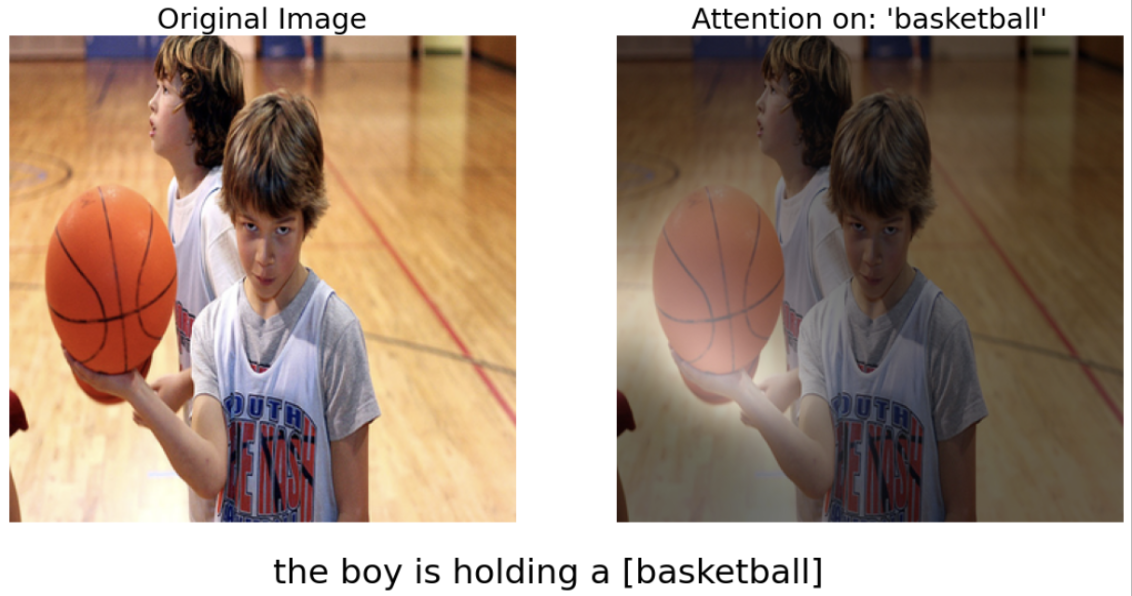
\includegraphics[width=0.35\linewidth]{example-boy.png}
    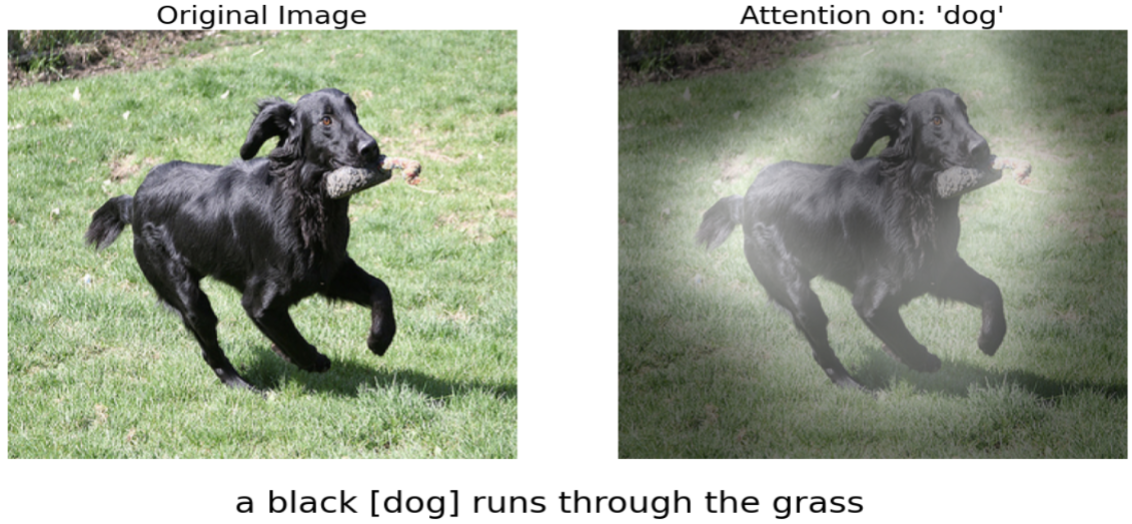
\includegraphics[width=0.4\linewidth]{example-dog.png}
    \caption{Soft attention from our re-implemented model [6]}
    \label{fig:results}
\end{figure}
Second, we replicated the BLEU and METEOR scores reported for the Flickr8k dataset under the soft attention model, aligning with Table 1 in the original paper. These metrics provide a quantitative measure of caption quality and serve as a benchmark for validating the fidelity of our re-implementation. 

Both results are central to the paper’s contributions, as they empirically validate attention as a mechanism for both improved performance and visual interpretability, which act as key advantages over prior image captioning models.

\section{Methodology}

Our re-implementation of the \textit{Show, Attend, and Tell} architecture was developed in modern PyTorch with CUDA acceleration for parallelized execution on NVIDIA GPUs. In our case, we used a Tesla T4, though any CUDA-compatible GPU is compatible. The system was modularly designed to support interchangeable CNN encoders and rapid prototyping of captioning components. While preserving the original model’s attention and decoder mechanisms, we adapted our training methodology to accommodate limited computational resources and enable reproducible experimentation with newer CNN architectures.

\begin{figure}[h]
    \centering
    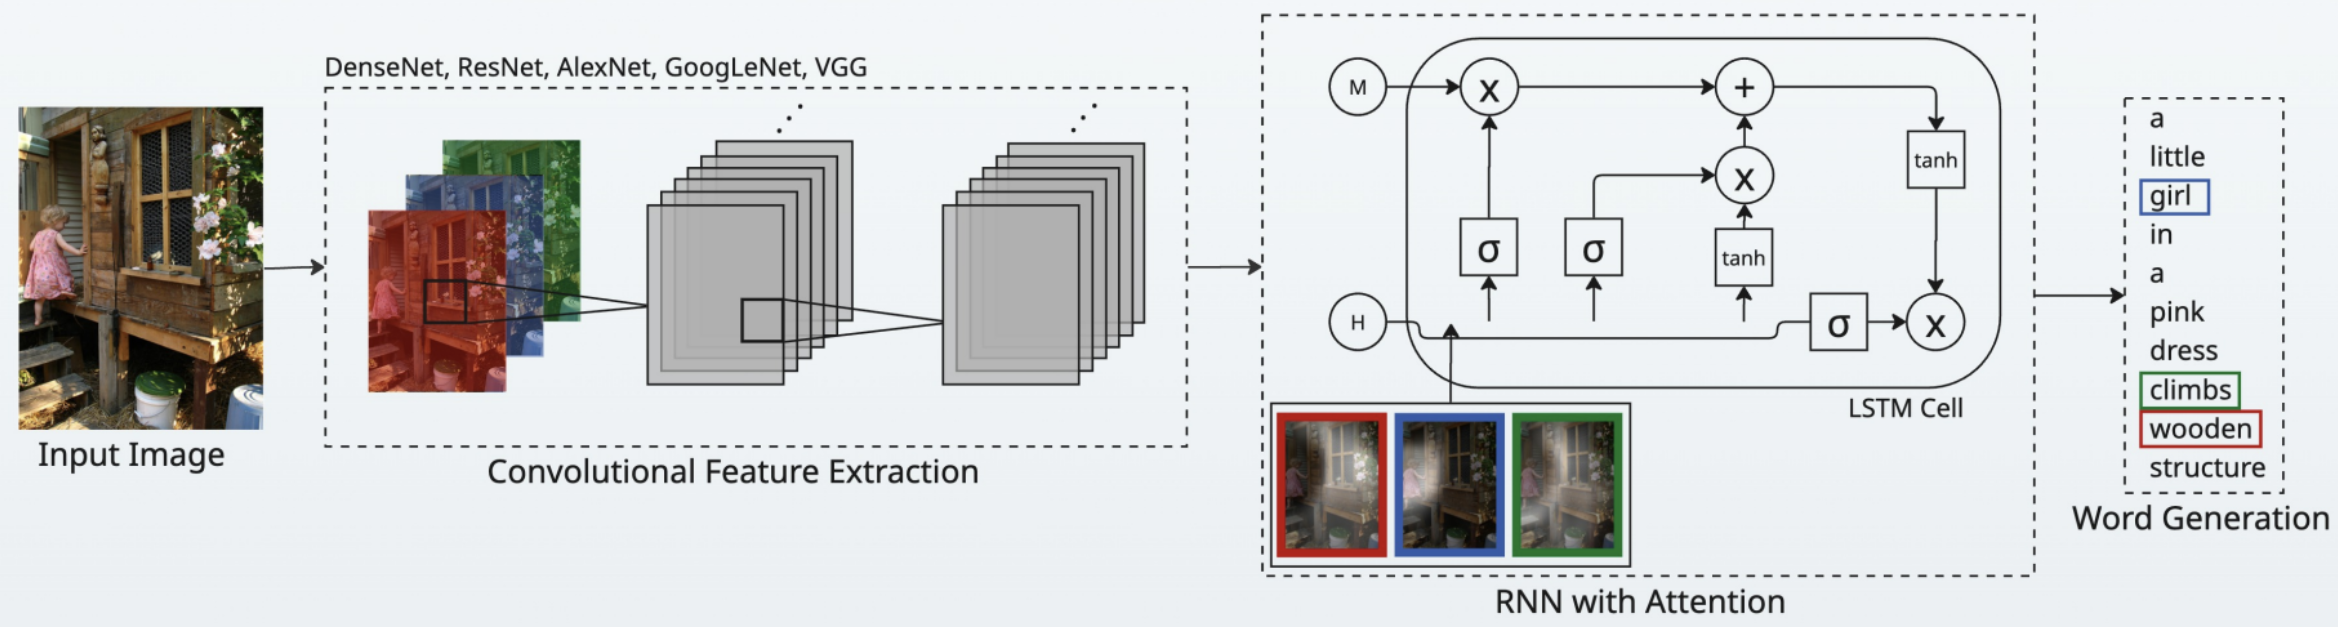
\includegraphics[scale=0.2]{methodology.png}
    \caption{Overall Model Architecture}
    \
\end{figure}
The model processes a single raw \textbf{input image} through a frozen, pre-trained CNN encoder, such as VGG, GoogLeNet, AlexNet, ResNet, or DenseNet, for \textbf{convolutional feature extraction}, where spatial features were extracted as annotation vectors. Including the original encoders from the paper (AlexNet, GoogleNet, VGG) ensured baseline comparability, while ResNet and DenseNet enabled evaluation of more recent architectures. ResNet mitigates the vanishing gradient problem via skip connections, supporting stable optimization in deeper architectures, while DenseNet promotes feature reuse and generalization through dense connectivity. These architectural modifications likely contributed to improved visual representation, even on our relatively small dataset.

The attention mechanism, implemented as part of the \textbf{RNN with Attention} module in Figure 2, assigns weights to annotation vectors to compute a context vector at each timestep. The paper proposed two variants: soft attention, which applies a softmax to produce a weighted sum, and hard attention, which samples a one-hot vector from a multinoulli distribution. The resulting context vector in hard attention reflects a sampled annotation location. Unlike soft attention, hard attention is non-differentiable and requires reinforcement learning for training. We chose not to implement it due to this reliance, which introduces additional complexity and potential instability during optimization.
 
In the LSTM decoder, initial memory and hidden states are computed by averaging the annotation vectors and passing them through two multilayer perceptrons. At each timestep, the decoder receives the context vector, previous word, and previous hidden state to generate the next word during the \textbf{word generation} step.

Unlike the original implementation trained on MS COCO for three days using a Titan Black GPU, we trained our soft attention model for 20 epochs using the Adam optimizer (learning rate 0.0001, batch size 32) on the smaller Flickr8k dataset. This choice reduced training time to around 2 hours, allowing for rapid experimentation. We used the dataset’s provided splits (6,000 images for training and 1,000 images each for validation and testing, with five human-annotated captions per image). Caption quality was evaluated using BLEU and METEOR scores on both training and validation sets across all five CNN encoders.

\section{Results and Analysis}
Our re-implementation achieved slightly lower BLEU and METEOR scores compared to the original soft attention model reported in Show, Attend and Tell for the Flickr8k dataset. We tested five frozen, pre-trained CNN encoders (AlexNet, GoogLeNet, VGG, ResNet, and DenseNet) and found that ResNet consistently performed the best, with BLEU-3 and METEOR scores closest to those in the original paper. As expected, ResNet and DenseNet outperformed older architectures like AlexNet, due to their deeper structure and design enhancements (e.g., residual and dense connections), which help preserve spatial features and mitigate vanishing gradients.
The performance gap between our best models and the original results was typically within 4\% across BLEU and METEOR scores. We attribute this to two primary factors: (1) the original paper fine-tuned its encoder during training, while our implementation used frozen pre-trained weights, and (2) we trained only on Flickr8k, a smaller dataset, to accommodate compute constraints. Frozen encoders, while computationally efficient, likely limited the model’s ability to learn image representations tailored specifically for captioning. The scores of our models and the original paper are shown in the table below.

\begin{table}[h]
\centering
\caption{Comparison of models on BLEU and METEOR scores.}
\label{tab:mytable}
\begin{adjustbox}{width=.75\textwidth}
\small
\begin{tabular}{lccccc}
\toprule
Model & BLEU-1 & BLEU-2 & BLEU-3 & BLEU-4 & METEOR \\
\midrule
Soft-Attention (Original Paper) & 67.0 & 44.8 & 29.9 & 19.5 & 18.93 \\
AlexNet                & 60.44 & 34.90 & 19.71 & 10.81 & 12.89 \\
DenseNet-201               & 64.81 & 40.82 & 26.26 & 15.84 & 16.95 \\
GoogLeNet (Inception-v1)              & 64.53 & 40.13 & 25.12 & 14.77 & 16.45 \\
VGG-19                    & 64.79 & 40.37 & 25.88 & 15.48 & 17.08 \\
ResNet-152                 & \textbf{65.67} & \textbf{41.40} & \textbf{27.13} & \textbf{16.48} & \textbf{17.94} \\
\bottomrule
\end{tabular}
\end{adjustbox}
\end{table}

In terms of qualitative performance, our model generated interpretable attention maps that closely aligned with the content and structure of the generated captions. As shown in Figure 3, the attention heatmaps track semantically relevant regions across time steps. For example, the model correctly focused on the "red" and "jeep" in corresponding image regions, and attended to background features such as the "rocky road" for relational terms like "on" which illustrated its ability to capture the fine-grained relationship between objects in the image, Notably, the model also allocated attention to non-object words such as “is” and “driving”, suggesting that it captures both objects and contextual relations. Overall, the model successfully learned to associate spatial features with linguistic outputs, reproducing one of the core strengths of the original approach. Based on the generated attention masks, our re-implemented model is capable of building a coherent visual-linguistic representation, grounding each word in relevant spatial context. 

\begin{figure}[h]
    \centering
    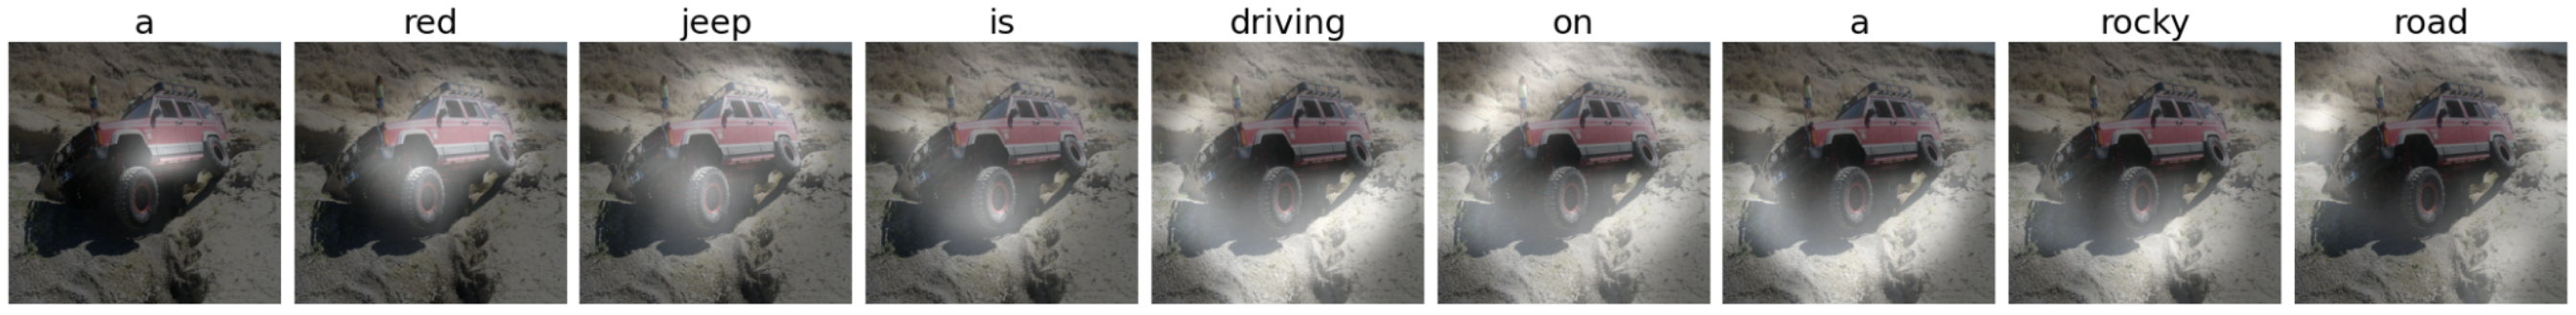
\includegraphics[width=0.75\linewidth]{example-jeep.png}
    \caption{Our model's attention mechanism visualization per word in generated caption.}
    \label{fig:enter-label}
\end{figure}

One of the primary challenges we faced during the re-implementation process was long training time. Training for just 10 epochs took nearly two hours on a Google Colab T4 GPU. To address this, we optimized the decoder code and added checkpoint saving to resume training across sessions. We ultimately trained soft attention models for 10–20 epochs across five encoder variants.

Another major challenge was the complexity of implementing hard attention. While we initially intended to implement both soft and hard attention, we decided to drop hard attention due to its reliance on reinforcement learning (REINFORCE), which increases training instability and resource demands. Given our time and hardware constraints, we prioritized soft attention as the more tractable and impactful component.

\section{Reflections}
Our re-implementation achieved meaningful results despite working with limited resources. Even though we trained on the smaller Flickr8k dataset and used frozen, pre-trained CNN encoders, the model was able to generate coherent captions and produce interpretable attention maps. This underscores the robustness and practicality of the soft attention mechanism, even in constrained settings.

One key lesson that we learned was the importance of setting feasible goals given time constraints and limited resources. Although the original paper explored both hard and soft attention mechanisms, we found that soft attention was more practical to implement and train due to its differentiable and deterministic nature. We abandoned hard attention since it relies on sampling-based methods like REINFORCE to handle non-differentiable operations, resulting in high-variance gradients and unstable training, which were impractical under our time constraints.

Overall, this project deepened our understanding of attention mechanisms in image captioning and provided practical experience in re-implementing a significant paper in vision-language research. For future work, we would explore training on larger datasets such as Flickr30k or MS COCO to improve generalization and caption diversity. We also hope to implement hard attention to investigate whether its sharper spatial focus leads to measurable gains. Lastly, fine-tuning the CNN encoder during training could help the model extract features more aligned with the captioning task, potentially closing the performance gap with the original implementation.


\section{References}
\noindent
[1] Xu, K., Ba, J., Kiros, R., Cho, K., Courville, A., Salakhutdinov, R., Zemel, R., \& Bengio, Y. (2015). Show, Attend and Tell: Neural Image Caption Generation with Visual Attention. Paper Website. \\ https://kelvinxu.github.io/projects/capgen.html\\

\noindent
[2] Xu, K. Arctic Captions: Theano Implementation of Show, Attend and Tell. GitHub repository. \\ https://github.com/kelvinxu/arctic-captions\\

\noindent
[3] Wong, A.. Show, Attend and Tell: PyTorch Implementation. GitHub repository. \\ https://github.com/AaronCCWong/Show-Attend-and-Tell\\

\noindent
[4] Hodosh, M., Young, P., \& Hockenmaier, J. (2013). Framing Image Description as a Ranking Task: Data, Models and Evaluation Metrics. Journal of Artificial Intelligence Research, 47, 853–899.\\ https://doi.org/10.1613/jair.3994\\

\noindent
[5] Paszke, A., Gross, S., Massa, F., Lerer, A., Bradbury, J., Chanan, G., ... \& Chintala, S. (2019). PyTorch: An Imperative Style, High-Performance Deep Learning Library. Advances in Neural Information Processing Systems, 32. \\ https://arxiv.org/pdf/1912.01703\\

\noindent
[6] Xu, K., Ba, J., Kiros, R., Cho, K., Courville, A., Salakhutdinov, R., Zemel, R., \& Bengio, Y. (2015). Show, Attend and Tell: Neural Image Caption Generation with Visual Attention. Proceedings of the IEEE Conference on Computer Vision and Pattern Recognition (CVPR), 2015.
https://arxiv.org/abs/1502.03044

\end{document}
